%----------------------------------------------------------------------------
\chapter{Evaluation}
%----------------------------------------------------------------------------
\section{Displaying the procedural program}
During development, and when running the finished tool, it became very important to see the output of the parser part in an easy to read form. The C\# debugger did not fit for that job, since despite that I could see the object hierarchy, and inspect values and statements one-by-one, I could not see the converted program as a whole. 

Therefore, I overrode the ToString functions for all the model objects to return an easy to read string reflecting its contents. After that, all I had to do was to call ToString on a \textit{Sequence} object, and it returned a pseudo-code of the converted program.

In the following examples, the shown converted procedural examples are the output of this routine.
\section{Small demos}
\paragraph{Demo "A"}
For the first demo I used the same program, which I used to demonstrate symbolic execution in the Background section (Listing \ref{lst:symbolic_test}). The dataflow counterpart of that program can be seen on Figure \ref{fig:testvi1}.
\begin{figure}
\centering
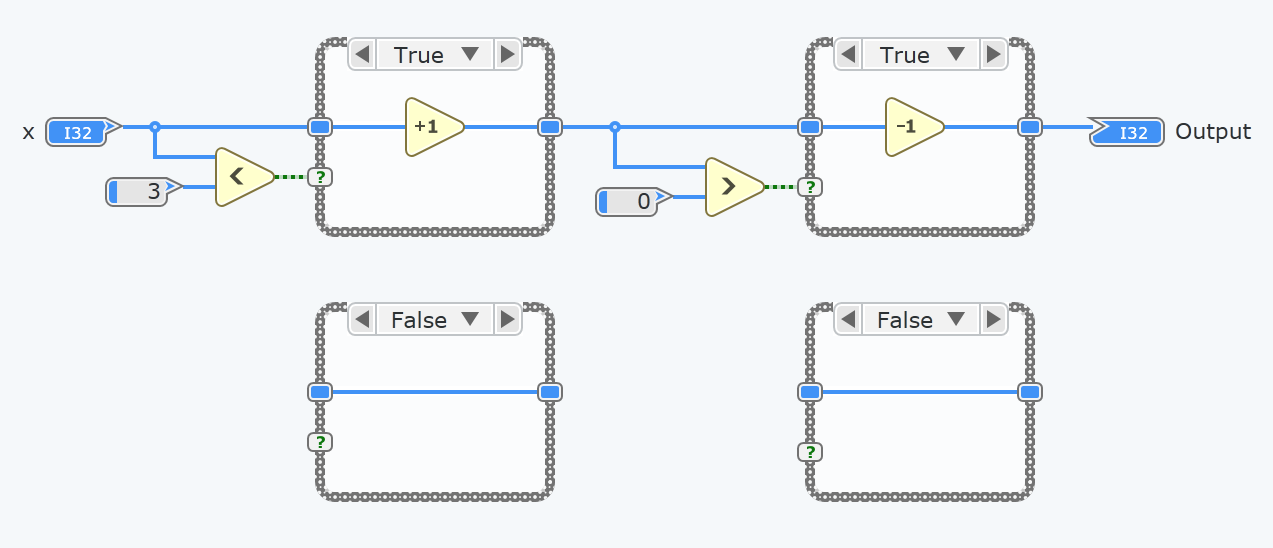
\includegraphics[width=150mm,keepaspectratio]{figures/testvi1.png}
\caption{Example VI "A"} 
\label{fig:testvi1}
\end{figure}

\begin{lstlisting}[frame=single,float=!ht,caption={The converted procedural version of VI "A"},captionpos=b,label={lst:testvi1_proc},language=]
A = [x]; 
B = 3; 
C = 0; 
D = (A < B); 
IF D Then
E = (A + 1); 
ELSE
E = A; 
End IF
F = (E > C); 
IF F Then
G = (E - 1); 
ELSE
G = E; 
End IF
[Output] : G; 
\end{lstlisting}

\begin{lstlisting}[frame=single,float=!ht,caption={The output of the symbolic execution for VI "A"},captionpos=b,label={lst:testvi1_sym},language=]
pc: (([x] < 3) & (([x] + 1) > 0)), x=0
pc: (([x] < 3) & !(([x] + 1) > 0)), x=-1
pc: (!([x] < 3) & ([x] > 0)), x=3
\end{lstlisting}

The outputs of symbolic execution in this example (Listing \ref{lst:testvi1_sym}) are the same as the expected (see Figure \ref{fig:symbolic_test}), and the unreachable fourth execution path $(!([x] < 3) \& !([x] > 0))$ is omitted from the list.

To verify the correctness of the results, I ran the VI with these inputs, to see if they really produce different execution paths. As seen on Figure \ref{fig:verify1}, all the possible paths have been covered with this input set.
\begin{figure}
\centering
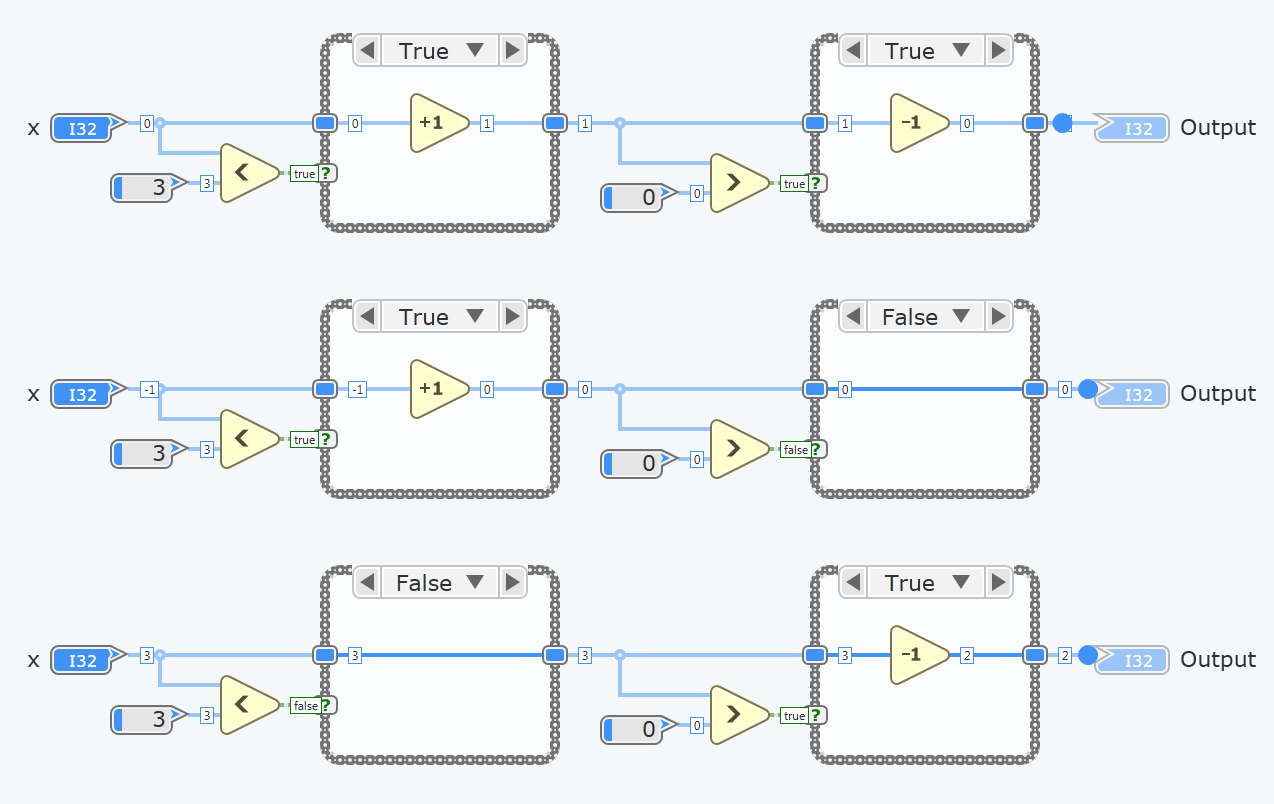
\includegraphics[width=140mm,keepaspectratio]{figures/verify1.png}
\caption{Run VI "A" with the result values as input} 
\label{fig:verify1}
\end{figure}

\paragraph{Demo "B"}
I wanted to test, if nesting case structures behaves correctly. When \textit{outside var} is false, \textit{inside var} should not matter in the path condition. Additionally, this test verifies, that boolean input values are processed correctly.

\begin{figure}
\centering
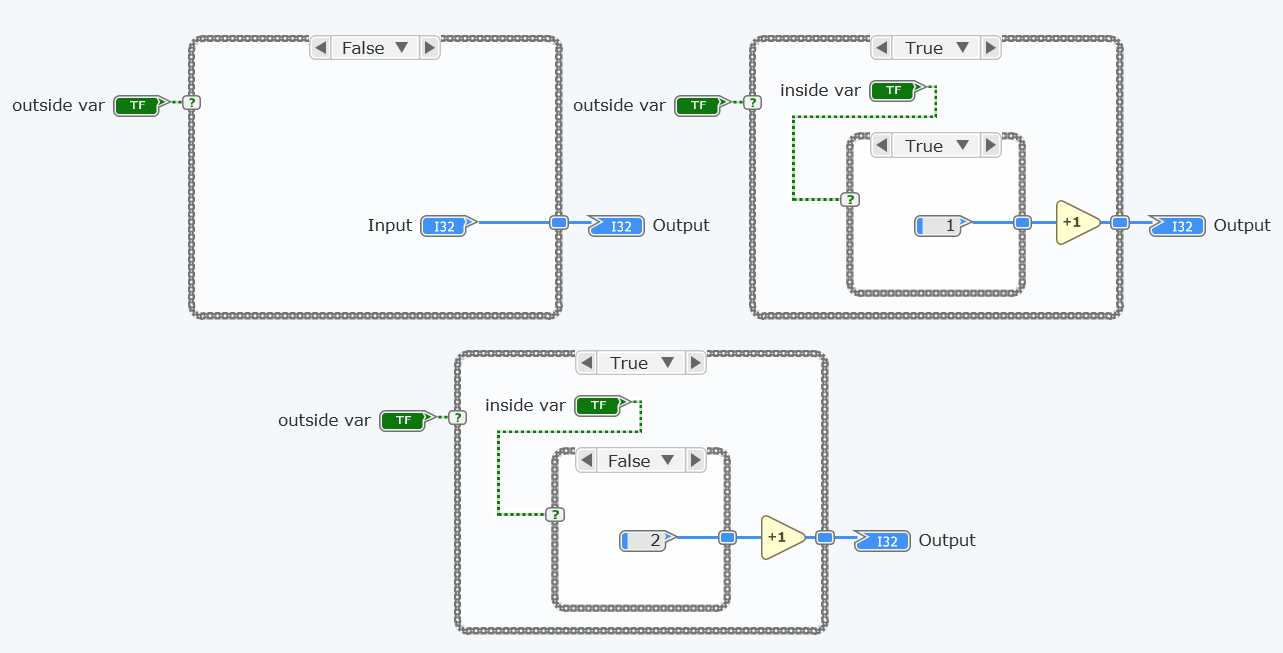
\includegraphics[width=150mm,keepaspectratio]{figures/testvi2.png}
\caption{Example VI "B"} 
\label{fig:testvi2}
\end{figure}


\begin{lstlisting}[frame=single,float=!ht,caption={The output of the symbolic execution for VI "B"},captionpos=b,label={lst:testvi1_sym},language=]
pc: ([outside var] & [inside var]), inside var=true, outside var=true
pc: ([outside var] & ![inside var]), inside var=false, outside var=true
pc: ![outside var], outside var=false
\end{lstlisting}

%% screenshots